\subsection{三视图}\label{subsec:czjh2-8-3}

\subsubsection{三视图的概念}

\begin{wrapfigure}[11]{r}{6cm}
    \centering
    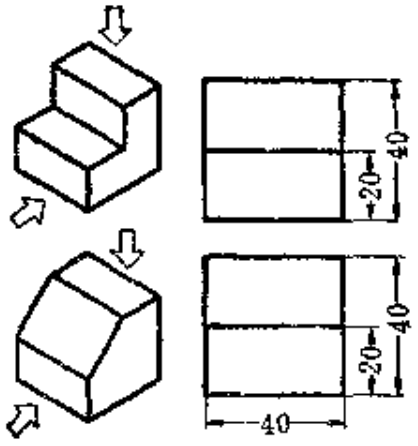
\includegraphics[width=5cm]{../pic/czjh2-ch8-12.png}
    \caption{}\label{fig:czjh2-8-12}
\end{wrapfigure}

有两个大小一样的正方体,棱长为 40 mm,分别切去一块,如图 \ref{fig:czjh2-8-12} 所示。
如果根据指定的方向画它们的二视图,两个几何体的二视图是完全一样的。
这就产生了一个问题,工人根据这样一张二视图的图纸,制造出哪个零件才算合格呢?
可见,对于一些比较复杂的几何体,当用二视图不能反映它的形状和大小时,
往往需要画三个视图或者更多的视图。这里我们只介绍三视图。

如图 \ref{fig:czjh2-8-13},三视图是一个几何体在三个互相垂直的投影面上同时进行正投影所得的三个视图。

除了在正面投影面 $V$ 和水平投影面 $H$ 上的视图外,还增加了在侧面投影面 $W$ 上的视图。
物体在侧面投影面 $W$ 上的视图称为\zhongdian{左视图}。
主视图、俯视图和左视图统称为\zhongdian{三视图}。

\begin{figure}[htbp]
    \centering
    \begin{minipage}[b]{7cm}
        \centering
        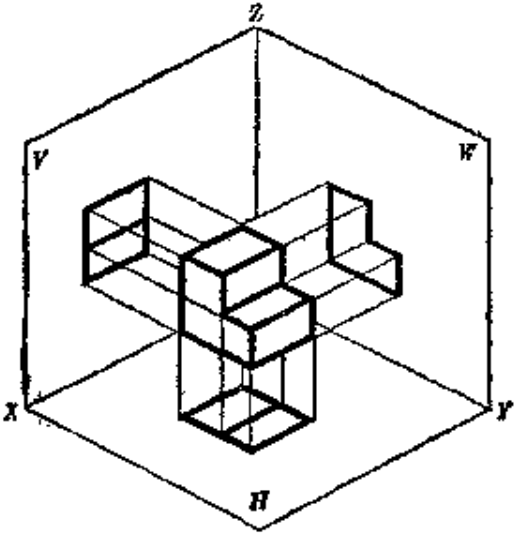
\includegraphics[width=6cm]{../pic/czjh2-ch8-13.png}
        \caption{}\label{fig:czjh2-8-13}
    \end{minipage}
    \begin{minipage}[b]{7cm}
        \centering
        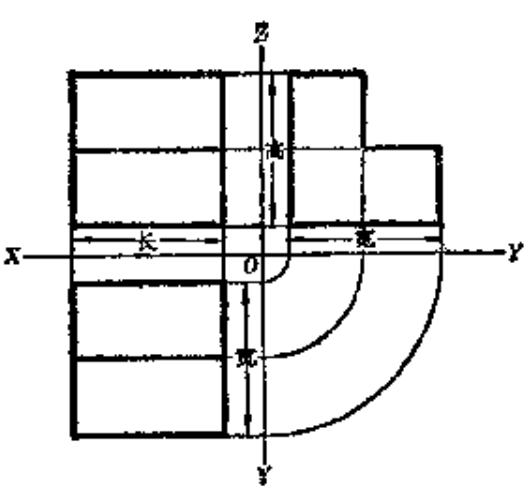
\includegraphics[width=6cm]{../pic/czjh2-ch8-14.png}
        \caption{}\label{fig:czjh2-8-14}
    \end{minipage}
\end{figure}

将几何体拿走后,把投影面 $H$ 向下转 $90^\circ$,投影面 $W$ 向后转 $90^\circ$,
使三个投影面摊平,三个视图就在同一个平面上,如图 \ref{fig:czjh2-8-14}。

三视图的位置是,俯视图在主视图的下面,左视图在主视图的右面。
主视图反映出物体的长和高,俯视图反映出物体的长和宽,左视图反映出物体的高和宽。

因此,三视图的画法规则可以归结为

\begin{center}
    \framebox{\zhongdian{长对正,宽相等,高平齐。}}
\end{center}


\subsubsection{三视图的画法}

我们以图 \ref{fig:czjh2-8-15} (a) 中的物体为例,说明三视图的画法,画图步骤如下:

\begin{figure}[htbp]
    \centering
    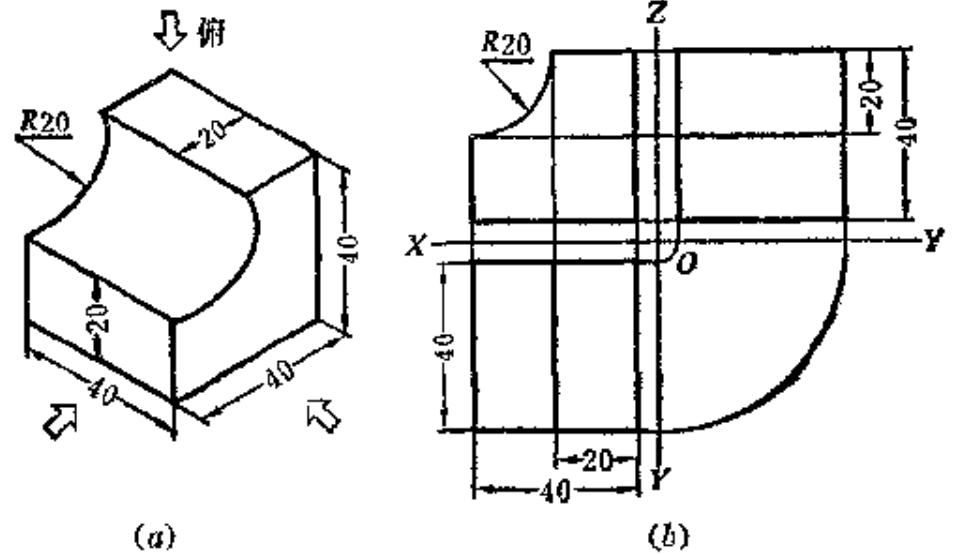
\includegraphics[width=11cm]{../pic/czjh2-ch8-15.png}
    \caption{}\label{fig:czjh2-8-15}
\end{figure}

(1)先画辅助轴线 $XY$、$YZ$ (图画好后可擦掉);

(2)确定主视图的位置,画出主视图;

(3)根据“长对正”与物体的宽度画出俯视图;

(4)再根据“高平齐”与“宽相等”画出左视图(宽度,可通过以点 $O$ 为中心的旋转画出);

(5)标注尺寸,擦去不必要的辅助线。

为了正确表达零件的内外形状,使图面清楚易读,绘图中使用的图线,即线型,应符合统一标准:
轮廓线用粗实线,看不见部分的轮廓线用虚线,尺寸线、尺寸界线用细实线,对称轴线用点划线,
等等(见本章\hyperref[sec:czjh2-8-fulu]{附录})。


\begin{lianxi}

\xiaoti{找出与下列几何体对应的三视图,在三视图下面的括号中填上对应的数码。}

\begin{figure}[H]
    \centering
    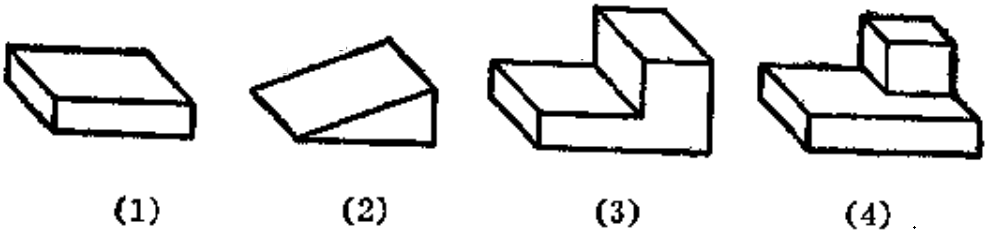
\includegraphics[width=11cm]{../pic/czjh2-ch8-subsec3-lx-01-1.png}
\end{figure}

\begin{figure}[H]
    \centering
    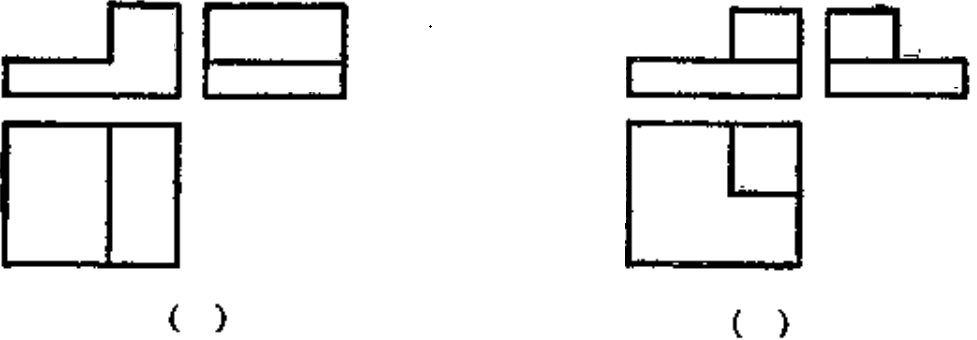
\includegraphics[width=10cm]{../pic/czjh2-ch8-subsec3-lx-01-2.png}
\end{figure}

\begin{figure}[H]
    \centering
    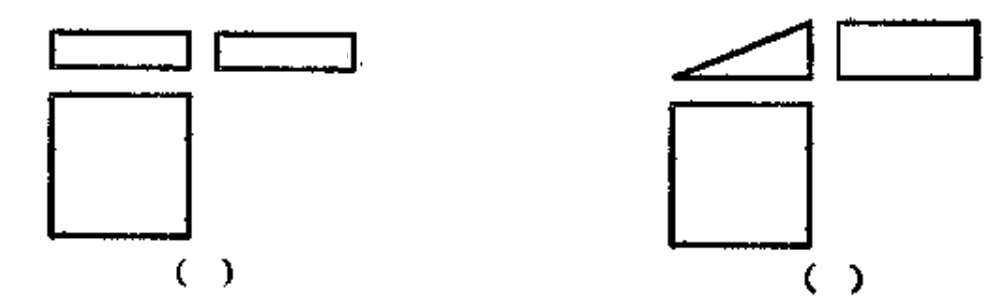
\includegraphics[width=10cm]{../pic/czjh2-ch8-subsec3-lx-01-3.png}
    \caption*{(第 1 题)}
\end{figure}

\xiaoti{添线补全下列三视图。}

\begin{figure}[htbp]
    \centering
    \begin{minipage}[b]{7cm}
        \centering
        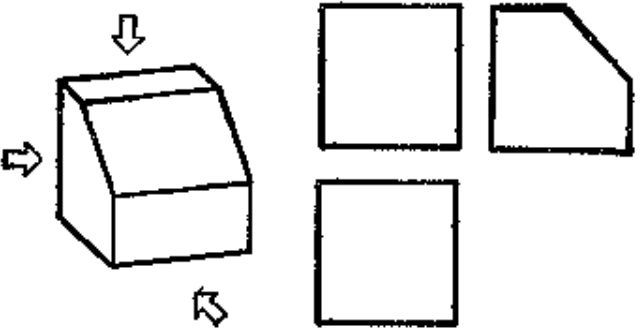
\includegraphics[width=6.8cm]{../pic/czjh2-ch8-subsec3-lx-02-1.png}
        \caption*{(1)}
    \end{minipage}
    \qquad
    \begin{minipage}[b]{7cm}
        \centering
        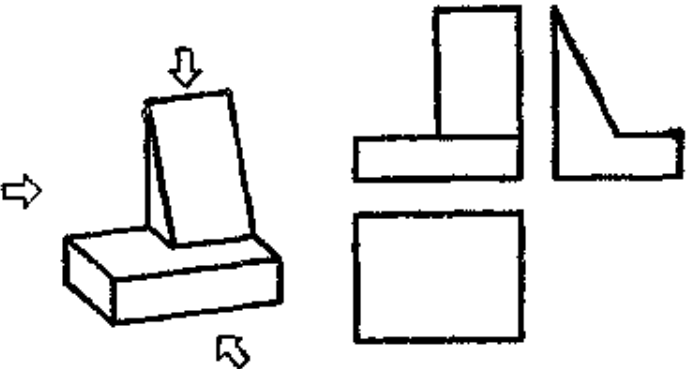
\includegraphics[width=6.8cm]{../pic/czjh2-ch8-subsec3-lx-02-2.png}
        \caption*{(2)}
    \end{minipage}
    \caption*{(第 2 题)}
\end{figure}


\xiaoti{画出下列几何体的三视图。}

\begin{figure}[htbp]
    \centering
    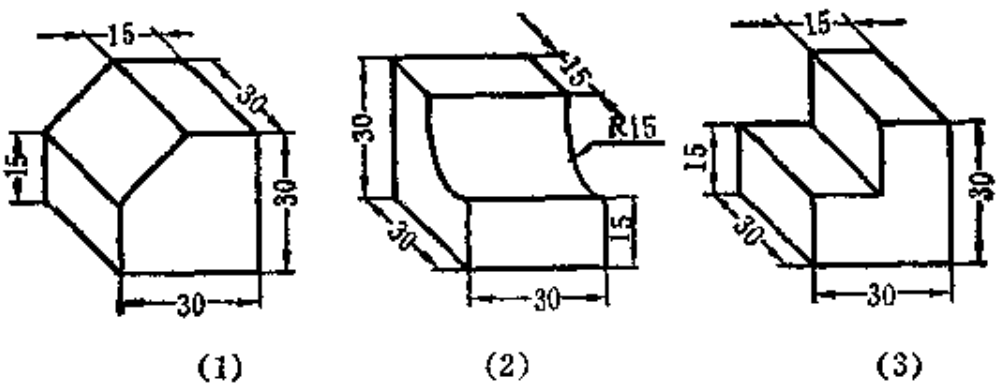
\includegraphics[width=11cm]{../pic/czjh2-ch8-subsec3-lx-03.png}
    \caption*{(第 3 题)}
\end{figure}

\end{lianxi}